\documentclass[prl,aps,superscriptaddress,twocolumn,11pt,nolongbibliography]{revtex4-2}
\usepackage[pdftex]{graphicx}
\usepackage{color}
\usepackage{amsmath,amsthm,amssymb,mathtools}
\usepackage[colorlinks=true,allcolors=blue]{hyperref}
\usepackage{enumerate}
\usepackage{sidecap}
\sidecaptionvpos{figure}{c}
\usepackage{soul}

% for inline codes
\usepackage{listings}
\usepackage{color}
\definecolor{codegreen}{rgb}{0,0.6,0}
\definecolor{codegray}{rgb}{0.5,0.5,0.5}
\definecolor{codepurple}{rgb}{0.58,0,0.82}
\definecolor{backcolour}{rgb}{0.95,0.95,0.92}
\lstdefinestyle{mystyle}{
    backgroundcolor=\color{backcolour},
    commentstyle=\color{codegreen},
    keywordstyle=\color{magenta},
    numberstyle=\tiny\color{codegray},
    stringstyle=\color{codepurple},
    basicstyle=\footnotesize,
    breakatwhitespace=false,
    breaklines=true,
    captionpos=b,
    keepspaces=true,
    numbers=left,
    numbersep=5pt,
    showspaces=false,
    showstringspaces=false,
    showtabs=false,
    tabsize=2
}
\lstset{style=mystyle}

\newcommand{\notes}[1]{\textbf{\textcolor[rgb]{1,0,0.5}{#1}}}
\newcommand{\mick}[1]{\textbf{\textcolor[rgb]{0,0.6,0.3}{#1}}}

\begin{document}
\title{CS 412: Project Proposal for Microbusiness Density Forecasting}
\author{Kittithat Krongchon (krongch2)}
\affiliation{Department of Physics, University of Illinois at Urbana-Champaign}
\author{Ting Cheng (tingc4)}
\affiliation{GIES College of Business}
\date{\today}

\maketitle

% Briefly introduce your task in the selected challenge. What is the input and what is the output?
% Getting to know your data. How large is it? What is the type of your data (categorical, numerical, etc)? 
% Are there any network, text or image data included?

\section{Introduction}
\begin{figure*}
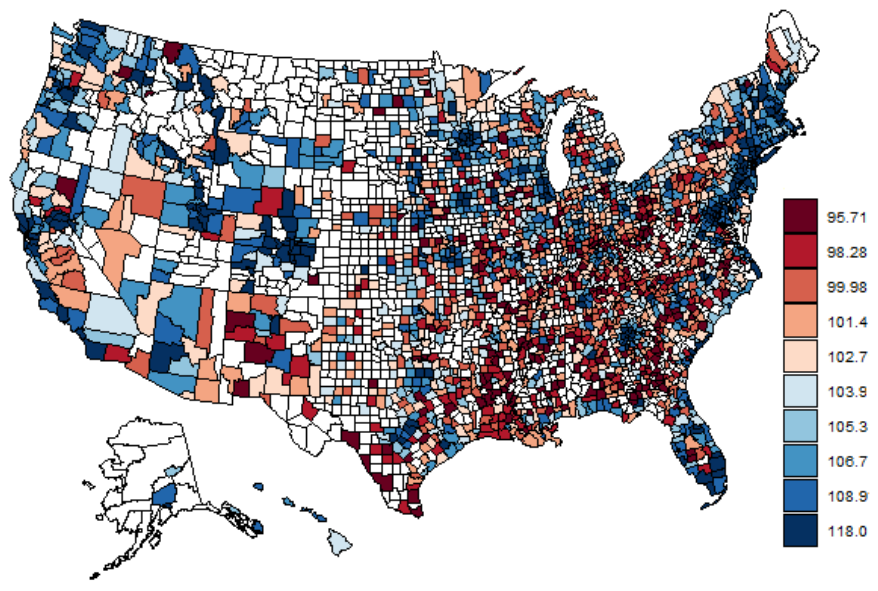
\includegraphics[width=5in]{figs/activity.png}
\caption{\label{fig:activity}
Microbusiness activity index by county in December 2021.
}
\end{figure*}

Policymakers in the United States attempt to create economies that are robust to industry downturns. 
The success (or limitation) of new policies heavily relies on the data of business entities. 
Gaining accurate visibility into enabling economic decisions, however, is a challenging task because a large number of `microbusinesses'', defined as businesses with ten or fewer employees, are often too small or too new to be included in standard data sources.
To overcome this challenge, the Venture Forward team at GoDaddy has studied tens of millions of microbusinesses in the United States for several years and has made the survey data publicly available. 
Thus, using data science techniques will enable policy leaders to gain more insights, which will be helpful for microbusiness entrepreneurs. 
This competition serves as a platform for participants to broaden the economic impact. 


\section{Data interpretation}
For the Microbusiness Density Forecasting project, the challenge is to predict the microbusiness density data in November 2022 based on the historical data from 2017 to 2021. The input data is, and our ouput is 
% Briefly introduce your task in the selected challenge. What is the input and what is the output?
We have three datasets which are training, testing and census starter data. The total size of these datasets is 10.93MB and all of them are numerical data without unstructured data. The censusstartern dataset, the training data, and the testing data
% Getting to know your data. How large is it? What is the type of your data (categorical, numerical, etc)? 
% Are there any network, text or image data included?

The task for this competition is to forecast microbusiness activity (Fig.~\ref{fig:activity}) across the United States, as measured by the density of microbusinesses for each of the 3142 counties. 
The values for this column are provided on a monthly basis, starting from August 1, 2019 to October 1, 2022. 
The participants are predicting the microbusiness density for the next month. 
Thus, the total number of given records is $3142 \times 39 = 122538$ rows of data.
The other columns that are provided include the percentage of households in the county with access to broadband of any type, the percent of the population in the county over age 25 with a 4-year college degree, the percent of the population in the county born outside of the United States, the percent of the workforce in the county employed in information related industries, and the median household income in the county. 
These extra columns serve as features in training models.


\section{Method}
Time Series model(ARIMA or GARCH) and ML models(linear regression, random forest, unsupervised learning)

Baseline Approach: SMAPE, RMSE
% How do you plan to solve it? Explain your idea at a high-level. (You may revise it or even propose a completely new one later. We just need to know that you have already spent some time thinking about it.)
% List at least 2 baseline approaches you would like to compare with. Add citations if they are from research papers.

\section{Timeline}
Timeline: Proposal:Feb 16th, Training data: ...

Feasibility: 
% A timeline that specifies your plan to finish the course project.
% Argue on the feasibility to finish the task on the selected challenge. If your framework is too complicated, you might struggle to implement it. Feel free to use existing tools and packages (e.g., repositories on GitHub).

\end{document}
